\section{Task 3}
Vorab erwähnt: Wir haben sowohl den Alpha-Beta Algorithmus als auch den MinMax Algorithmus angepasst, dass dieser beim Überschreiten einer Zeitvorgabe sofort terminiert und den TimeOut auch im Rückgabewert kenntlich macht. Dafür haben wir ausgenutzt, dass unsere Bewertungsfunktion im Wertebereich  $(0,100)$  liegt. Den negativen Werten konnten wir dementsprechend eine besondere Bedeutung geben.\\
Nun kommen wir zum Iterative Deepening Algorithmus, in diesem Report als 'Deepener' bezeichnet.
Der Deepener ist implementiert in der Klasse IterativeDeepeningCalculator, welcher selber keine Kalkulation durchführt sondern diese Arbeit an einen anderen Calculator delegiert.

\begin{figure}[h]
	\begin{center}
		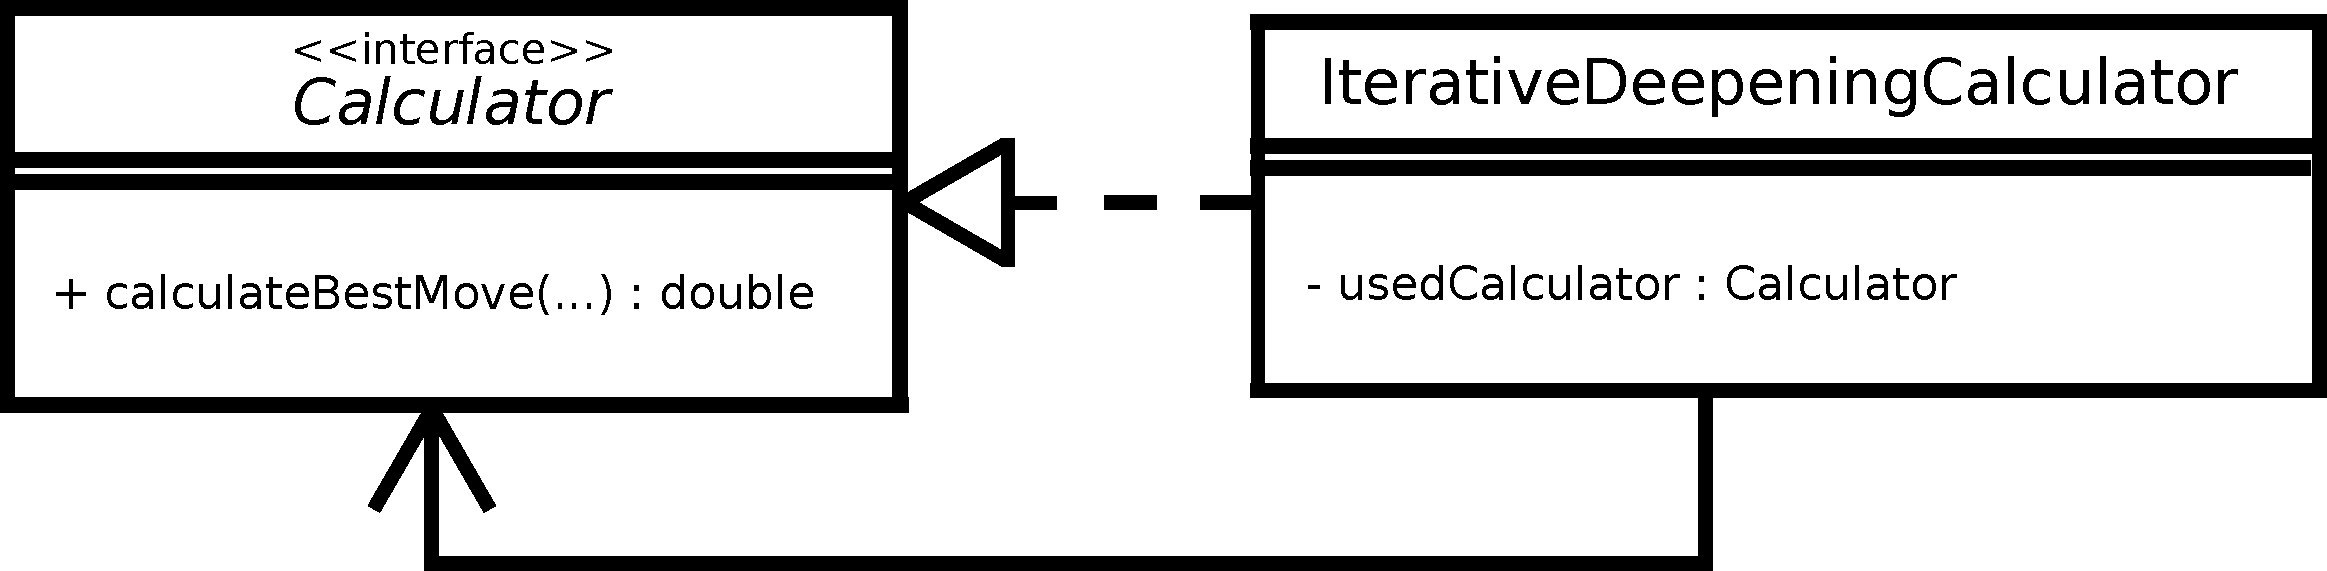
\includegraphics[scale=0.4]{deepener-classdiagram}
		\label{fig::IterativeDeepeningCalculator-classdiagram}
		\caption{Klassendiagramm von IterativeDeepeningCalculator}
	\end{center}
\end{figure}
Dabei erhält jeder Calculator ein "Formular" (Klasse CalculatorForm), welcher er beim Aufruf von $calculateBestMove()$ ausfüllen muss. Diese Informationen sind als Schnittstelle zu den aufrufenden Klassen gedacht. In dem Formular wird momentan der beste Zug, der maximale Verzweigungsgrad und ob der Algorithmus bis zum Ende der Spielphase gerechnet hat, hinterlegt. Diese Informationen nutzt der Deepener um effizienter mit der Bedenkzeit umzugehen. Seine Arbeitsweise ist in Abbildung \ref{fig::Deepener-Flow-Chart} als Flussdiagramm gezeigt.\\
\begin{figure}[h]
	\begin{center}
		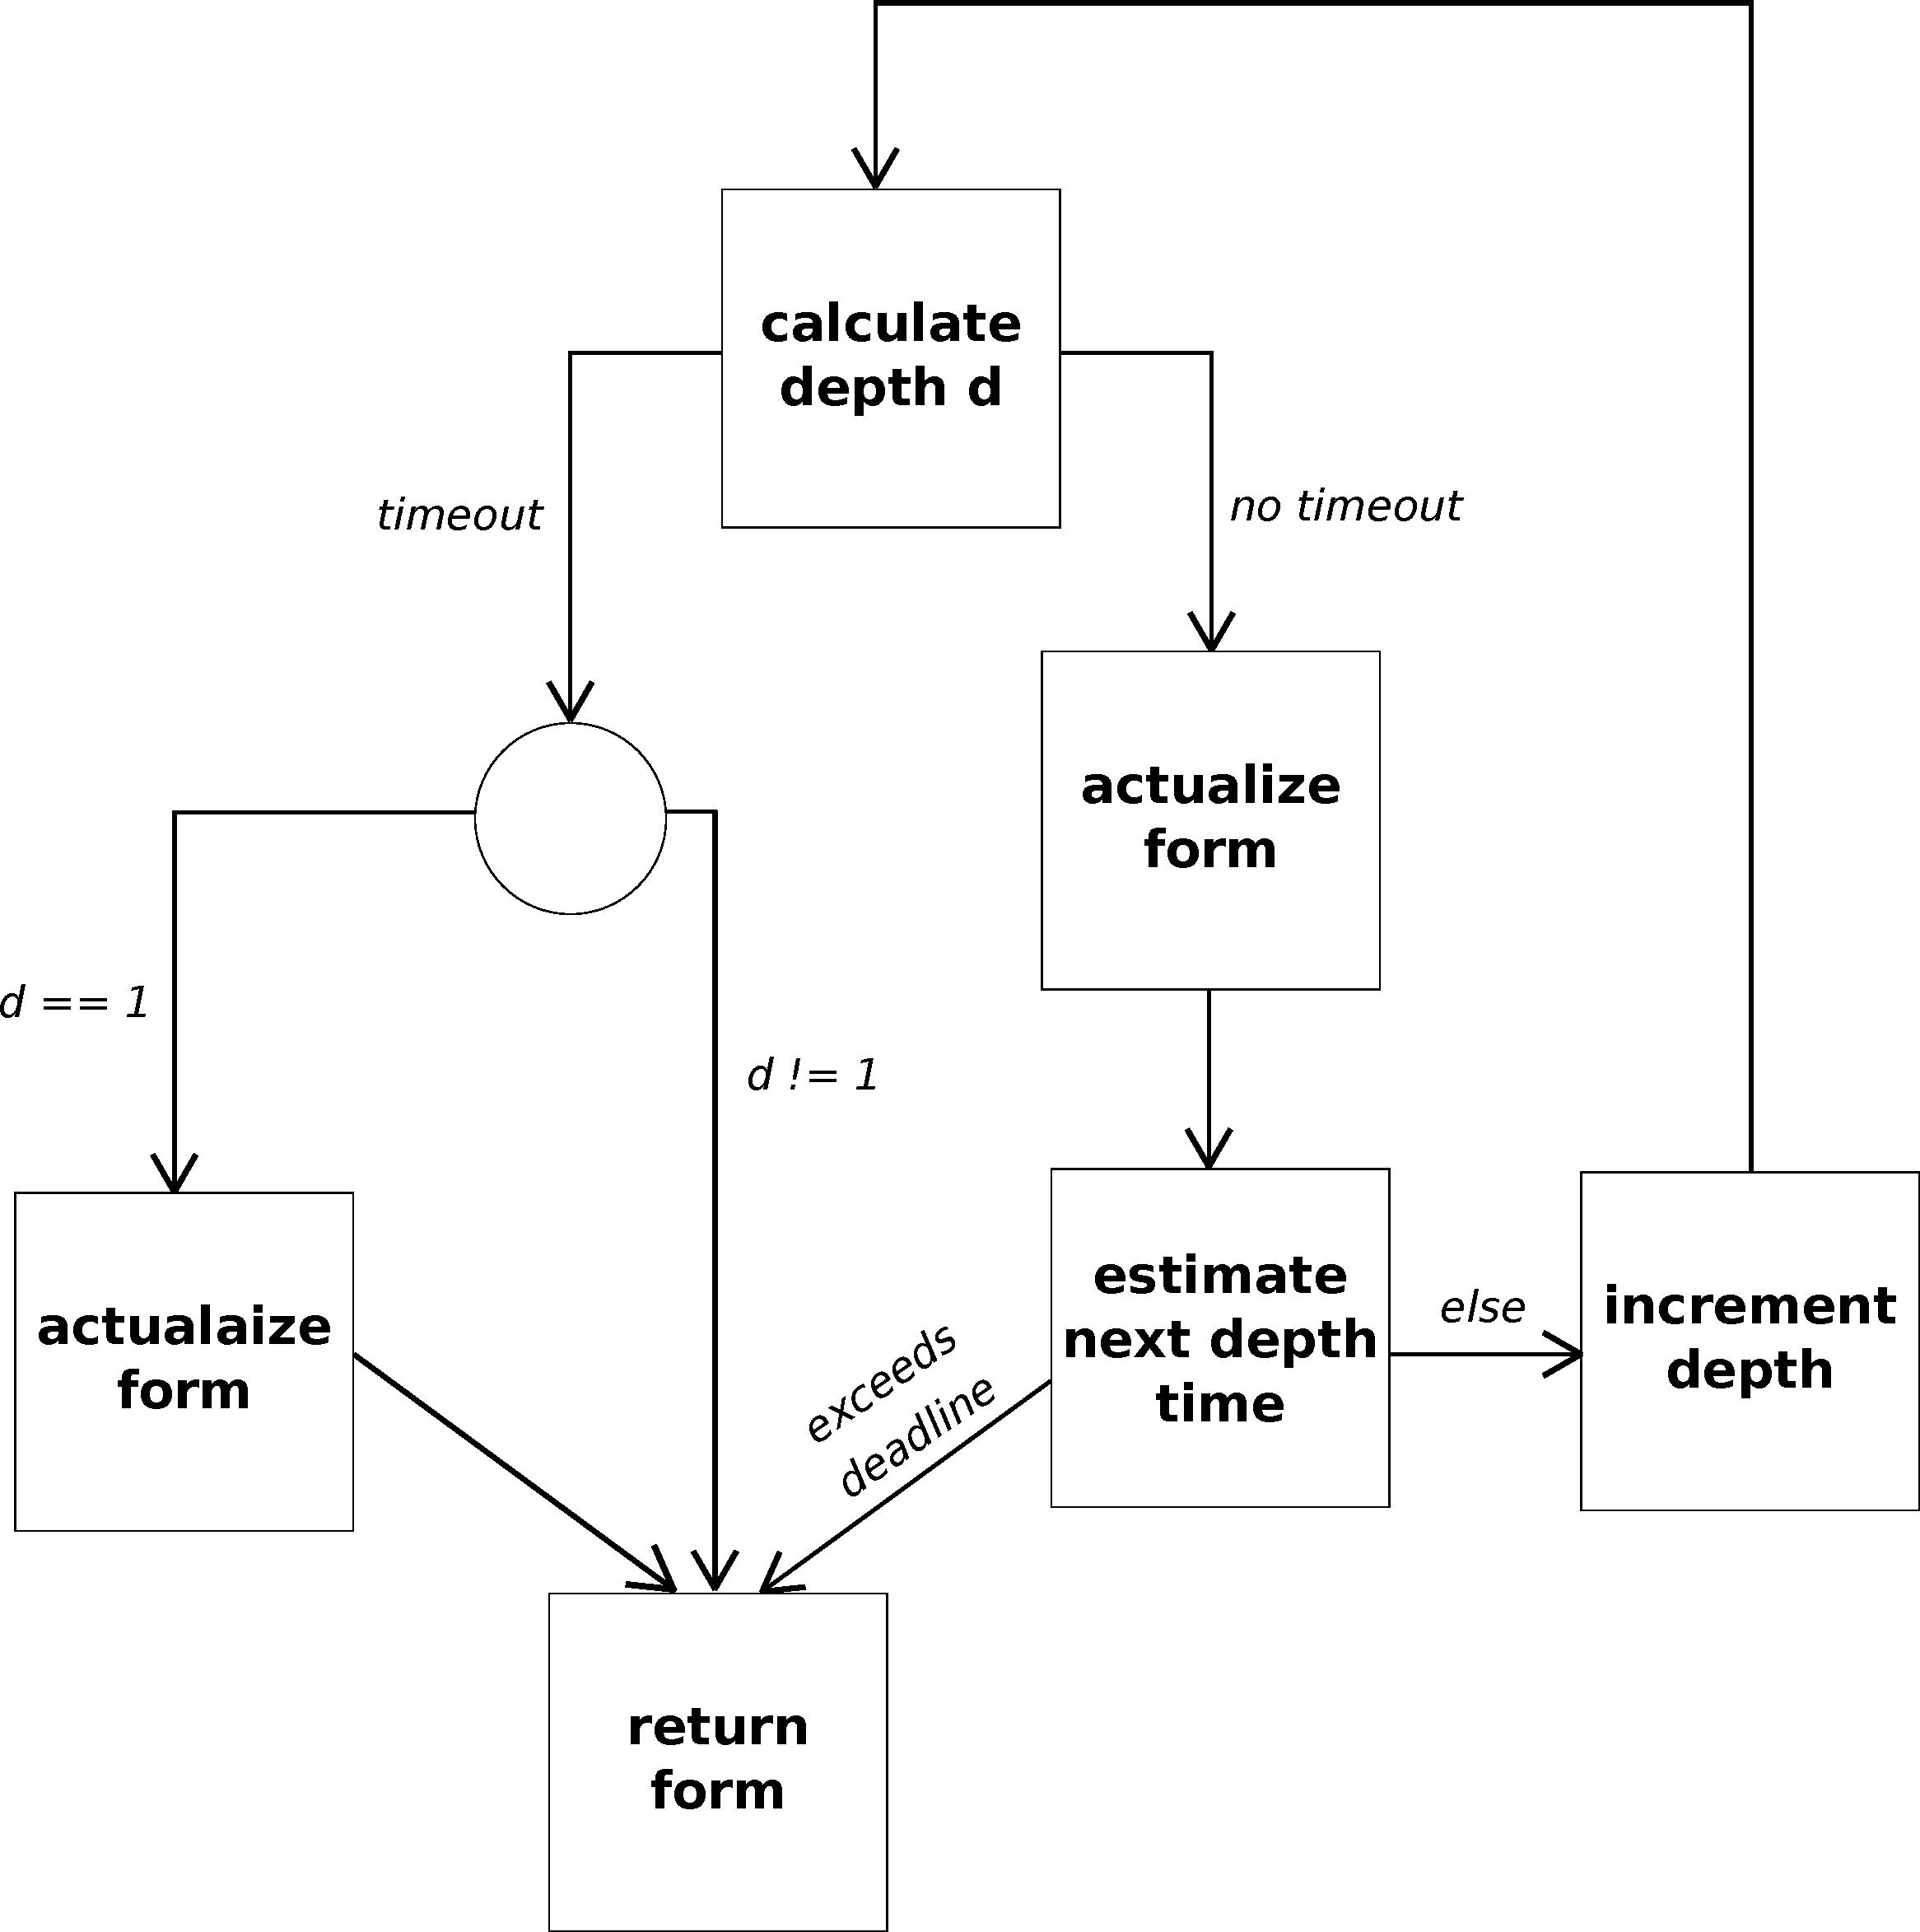
\includegraphics[scale=0.3]{deepener-flow-chart}
		\label{fig::Deepener-Flow-Chart}
		\caption{Programmfluss vom Deepener}
	\end{center}
\end{figure}
Für die Zeitabschätzung der nächsten Tiefe der maximale Verzweigungsgrad $k_{max}$ genutzt. Da die meiste Zeit der Kalkulation in den Blättern steckt und deren Anzahl sich in einem gleichmäßigen Variantenbaum um den Verzweigungsgrad vervielfacht ist die geschätzte Zeit für Tiefe $d+1$:
\begin{equation*}
	t(d+1) = t(d) * k_{max}
\end{equation*}
Dies ist eine einfache aber unter Umständen sehr konservative Abschätzung, gerade weil der Verzweigungsgrad nicht die Anzahl besuchter Teilbäume beschreibt (im Alpha-Beta können diese teilweise abgeschnitten werden). Außerdem wird außer Acht gelassen, dass man mit den Ergebnissen des Deepeners aus der vorhergehenden Tiefe eine bessere Zugsortierung machen kann um den Effekt des Alpha-Beta-Prunings zu verstärken und somit denselben Variantenbaum in kürzerer Zeit auskundschaften zu können.